\subsection{系统性能测试}
\label{subsec:featurespy-evaluation-performance}

\paragraph*{测试环境。} 本文为\prototype 的性能评估配置了以下两个测试平台:

\begin{itemize}[leftmargin=*]
    \item {\bf 本地集群(LAN)。}包括三台设备,每台设备均配备一个八核2.9\,GHz的Intel Core i7-10700 CPU,一个4\,TB 7200转的希捷银河系列SATA机械硬盘32\,GB DDR4内存。所有机器都通过10\,Gbps交换机进行连接,并运行Ubuntu 20.04.3 LTS。
    \item {\bf 云环境(Cloud)。}本文在两个不同区域的阿里云\cite{Alibaba}部署了多台规格为{\em ecs.g7t.3xlarge}的虚拟机(VM)来分别运行云服务端、密钥服务器和多个客户端。同一地域和不同地域的虚拟机分别通过10\,Gbps和100\,Mbps网络连接。每个虚拟机均配备一个12核3.5GHz的虚拟CPU(底层物理机CPU为Intel Xeon (Ice Lake) Platinum 8369B)和48GiB内存,并安装阿里云Linux 3.2104操作系统。本文另外挂载了阿里云通用存储{\em Alibaba General-Purpose NAS}作为云服务端的存储后端。该NAS可实现高达15K\,IOPS的4\,K随机读写,且顺序读写性能为150\,MB/s。
\end{itemize}

本文进行以下默认配置:对于底层\sysnameF,本文固定检测窗口大小$W$=5\,K(需消耗大约300\,KiB安全区内存),报告攻击的阈值$T$=3\%,相似性指标的大小为2个加密块(即,32字节),通过N-transform提取的特征数量为3个。对于\prototype,本文配置了三个线程来提取明文数据块的内容特征(除了 Exp\#5,它使用单个线程对\prototype 中各个模块的性能进行基准测试,而 Exp\#6评估了\prototype 使用不同线程数进行特征提取时的性能),并在云服务端使用了一个大小为1\,GiB容器(云服务端的基本存储单位,参见\S\ref{sec:featurespy-implementation})缓存以提高下载性能。

\subsubsection{合成数据集工作负载}
\label{subsec:featurespy-syn}
本文使用SYNUnique评估\prototype 在合成数据集作为工作负载情况下的性能。数据集中每个2\,GiB的随机文件均只包括全局非重复的数据块(\S\ref{subsec:featurespy-datasets})。为了测试\prototype 的峰值性能,本文在每次测试之前将所有数据加载到每个客户端的内存中(避免磁盘I/O的影响),并将云服务端接收到的所有数据存储在内存中(不包含Exp\#8,其包含磁盘I/O以研究真实云环境部署下的系统性能)。实验结果表明\prototype 与本文提出的高性能加密重复数据删除系统\sysnameS (\S\ref{sec:sgxdedup-implementation})相比仅产生有限的性能开销。本文将每个实验的10次测试的平均结果及其T分布{\em Student's t-Distribution}95\%置信区间包含在条形图中(为简洁起见,折线图中不包含置信区间)。

\paragraph*{Exp\#5(微基准性能测试)。}
本文通过微基准测试了解\prototype 中各个步骤的计算开销。本实验在LAN测试平台的不同机器上分别部署客户端、密钥服务器和云服务端。本文使用客户端连续上传两次SYNUnique中的同一个2\,GiB随机文件,并在单个线程中评估不同步骤的处理时间。本文考虑的步骤包括:(1)数据分块({\em chunking}),将输入文件划分为可变大小的明文数据块;(2)特征提取({\em feature generation}),提取每个明文数据块的内容特征,并根据\sysnameF 的各个实例对目标特征进行采样;(3)数据块指纹计算({\em fingerprinting}),计算每个明文数据块的指纹;(4)密钥生成({\em key generation}),生成特征密钥和消息锁加密密钥;(5)加密({\em encryption}),对每个明文数据块进行保留相似性加密;(6)攻击检测({\em detection}),基于密文数据块的相似性指标检测推测内容攻击;(7)数据所有权证明({\em PoW}),证明每个密文数据块的所有权;(8)重复数据删除({\em deduplication}),云服务端检测数据块是否已被存储,并将结果返回给客户端;(9)数据传输({\em transfer}),传输不重复的密文数据块和文件元数据。

\begin{table}[!htb]
    \small
    \centering
    \setlength{\tabcolsep}{5pt}
    \renewcommand{\arraystretch}{1.05}
    \setlength{\tabcolsep}{0.006\textwidth}{
    \begin{tabular}{|c|c|c|c|c|}
        \hline
        \multicolumn{2}{|@{\,}c|}{\textbf{Procedure/Step}} & \multicolumn{1}{l|}{\hspace{.5em}\textbf{firstFeature}} &
        \multicolumn{1}{c|}{\textbf{minFeature}} &
        \multicolumn{1}{c|}{\textbf{allFeature}} \\ \hline \hline
        \multicolumn{2}{|c|}{Chunking} & \multicolumn{3}{c|}{$2.12\pm0.006$} \\ \hline
        \multicolumn{2}{|c|}{\makecell[c]{Feature generation}} &
        \makecell[c]{$4.34 \pm 0.01$} & \makecell[c]{$9.93 \pm0.04$} & \makecell[c]{$9.85 \pm0.02$} \\ \hline
        \multicolumn{2}{|c|}{\makecell[c]{Fingerprinting}}&
        \multicolumn{3}{c|}{$1.81 \pm 0.002$} \\ \hline        \multicolumn{2}{|c|}{\makecell[c]{Key generation}}&
        \multicolumn{3}{c|}{$0.73 \pm 0.02$ ($0.49 \pm 0.01$)} \\ \hline
        \multicolumn{2}{|c|}{Encryption} & \multicolumn{3}{c|}{$1.22 \pm 0.001$} \\ \hline
        \multirow{2}{*}{In Enclave}
        & Detection &
        \multicolumn{3}{c|}{$0.04   \pm 0.005$} \\ \cline{2-5}
        & PoW &
        \multicolumn{3}{c|}{$1.86   \pm 0.004$} \\ \hline
        \multicolumn{2}{|c|}{Deduplication}  &
        \multicolumn{3}{c|}{$0.55 \pm 0.02$}  \\ \hline
        \multicolumn{2}{|c|}{Transfer}  & \multicolumn{3}{c|}{$1.16 \pm 0.03$ ($0.04 \pm 0.001$)}\\ \hline
    \end{tabular}
    }
    \caption{(Exp\#5) 处理随机文件数据每 1\,MiB 的时间分解(单位:ms)。 除括号中明确指定外,第二次上传的每一步所消耗的时间与第一次上传的相同。}
    \label{tab:featurespy-evaluation-syn-system-breakdown}
\end{table}
表~\ref{tab:featurespy-evaluation-syn-system-breakdown} 展示了结果(每 1\,MiB 文件数据处理)。由于 \prototype 建立在 \sysnameS \cite{ren21} 之上,它继承了在第二次上传中卸载密钥生成 (\S\ref{sec:featurespy-implementation}) 的计算开销以及避免传输重复块的性能优势.检测步骤是高效的,并且在上传过程中占用了总时间的 0.4\%。此外,由于 N-transform的计算开销,特征生成步骤很昂贵。例如,{\tt firstFeature} 在第一次上传时占用了总时间的 31.4\%; {\tt minFeature} 和 {\tt allFeature} 所消耗的时间分数分别进一步增加到 51.1\% 和 50.9\%,因为它们提取了所有三个特征(与只提取第一个特征的 {\tt firstFeature} 相反) )。然而,本文认为本文可以通过多线程来减轻特征生成的性能开销(见下文)。


\paragraph*{Exp\#6(单客户端性能)。}
本文考虑单个客户端,并将 \prototype 的性能与基本系统 \sysnameS 进行比较。本文让客户端两次上传相同的文件(如 Exp\#5)并进一步下载文件。


图~\ref{fig:featurespy-singleClientThroughput}(a) 和Figure~\ref{fig:featurespy-singleClientThroughput}(b) 分别展示了当本文改变提取特征的线程数(\S\ref{sec:featurespy-implementation})。 \sysnameS 的速度在第一次上传时保持为 297.1\,MiB/s,在第二次上传时保持为 304.3\,MiB/s,因为它不提取特征。 \prototype 的上传速度首先随着线程数的增加而增加(例如,{\tt firstFeature} 为 265.3\,MiB/s,{\tt minFeature} 为 261.3\,MiB/s,{\tt minFeature} 为 262.6\,MiB/s {\tt allFeature} 当三个线程用于在第一次上传中提取特征时),然后减少(例如,在第一次上传中大约为 220\,MiB/s 和在第二次上传中为 225\,MiB/s 对于所有三个实例)由于资源争用。通过利用多线程,\prototype 仅在第一次上传时比 \sysnameS 产生 8.0-12.0\% 的性能开销,在第二次上传时为 6.6-7.5\%。此外,本文观察到第一次和第二次(不需要传输重复数据)上传之间的性能差异很小,因为本文的 LAN 测试平台具有高带宽来传输数据。本文认为源端重复数据删除在实际云部署中带来了显着的性能提升(Exp\#8),并减少了处理实际存储工作负载的网络流量(Exp\#10)。图~\ref{fig:featurespy-singleClientThroughput}(c)比较下载速度。 \prototype 会导致 1.3\% 的性能下降,因为它使用 MLE 密钥和特征密钥解密每个块。


\begin{figure}[!htb]
    \centering
    
\includegraphics[width=0.7\textwidth]{pic/featurespy/plot/performance/LANSyn/legend.pdf}\\
    \vspace{1pt}
    \begin{tabular}{@{\ }c@{\ }c@{\ }c}
        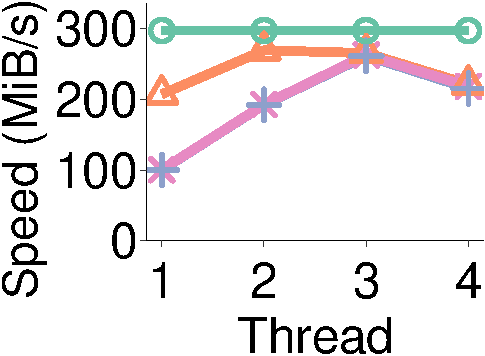
\includegraphics[width=0.32\textwidth]{pic/featurespy/plot/performance/LANSyn/upload_thread_line.pdf}&
        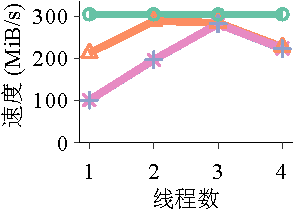
\includegraphics[width=0.32\textwidth]{pic/featurespy/plot/performance/LANSyn/upload_thread_2nd_line.pdf}&
        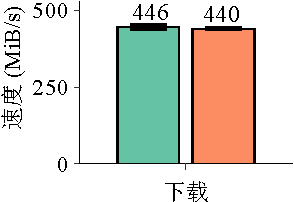
\includegraphics[width=0.32\textwidth]{pic/featurespy/plot/performance/LANSyn/download_bar.pdf}\\
        \makecell[c]{\small (a)第一轮上传} &
        \makecell[c]{\small (b)第二轮上传} &
        \makecell[c]{\small (c)下载}\\
    \end{tabular}
    \caption{(Exp\#6) LAN 测试平台中的单客户端性能。 在下载中,所有 \prototype 实例都达到相同的速度,本文将它们(橙色)与 \sysnameS(绿色)进行比较。}
    \label{fig:featurespy-singleClientThroughput}
\end{figure}

\paragraph*{Exp\#7(多客户端性能)。}
本文评估多个客户端同时发出上传/下载时的性能。 本文使用云测试台来考虑越来越多的客户端,并将所有客户端、密钥服务器和云部署在同一个区域。 本文将 {\em 聚合上传(下载)速度}衡量为总上传(下载)数据大小与所有客户端完成上传(下载)总时间的比率。

\begin{figure}[!htb]
    \centering
    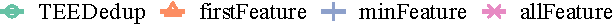
\includegraphics[width=0.7\linewidth]{pic/featurespy/plot/performance/multiClient/legend.pdf}\\
    \vspace{1pt}
    \begin{tabular}{@{\ }c@{\ }c@{\ }c}
            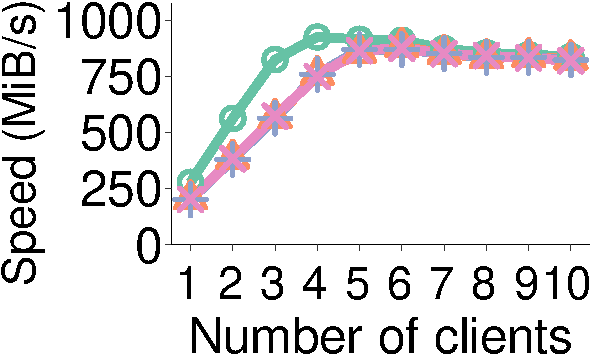
\includegraphics[width=0.32\textwidth]{pic/featurespy/plot/performance/multiClient/upload_1st_line.pdf}&
            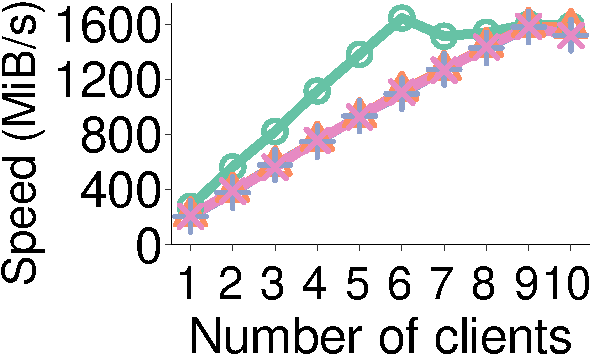
\includegraphics[width=0.32\textwidth]{pic/featurespy/plot/performance/multiClient/upload_2nd_line.pdf}&
            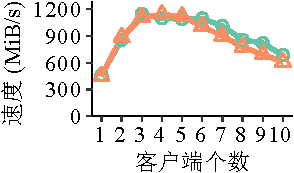
\includegraphics[width=0.32\textwidth]{pic/featurespy/plot/performance/multiClient/download_line.pdf}\\
            \makecell[c]{\small (a)第一轮上传} &
            \makecell[c]{\small (b)第二轮上传} &
            \makecell[c]{\small (c)下载}\\
        \end{tabular}
        \captionof{figure}{(Exp\#8) 多客户端性能。 所有 \prototype 实例的下载速度都是相同的,本文将它(橙色)与 \sysnameS(绿色)进行比较。}
        \label{fig:featurespy-expMultiClientThroughput}
\end{figure}

\begin{table}[!htb]
    \centering
    \small
    \begin{tabular}{cccc}
        \toprule
        {\bf 方案} & {\bf 第一轮上传(非重复数据)} & {\bf 第二轮上传(重复数据)} & {\bf 下载} \\
        \midrule
        网络带宽 & \multicolumn{3}{c}{11.8 $\pm$ 0.04} \\
        \makecell[c]{\tt firstFeature} & \multirow{3}{*}{11.5 $\pm$ 0.006} & 204.4 $\pm$ 10.06 & \multirow{3}{*}{11.5 $\pm$ 0.004} \\
        \makecell[c]{\tt minFeature} &  & 184.7$\pm$ 7.4 &  \\
        \makecell[c]{\tt allFeature} &  & 185.0$\pm$ 6.4 &  \\
        \sysnameS & 11.5 $\pm$ 0.009 & 233.2 $\pm$ 8.4 & 11.5 $\pm$ 0.004 \\
        \bottomrule
    \end{tabular}
    \captionof{table}{(Exp\#7) 云环境下部署\prototype 的上传/下载性能(单位:MiB/s)}
    \label{tab:featurespy-expCloudTest}
\end{table}

图~\ref{fig:featurespy-expMultiClientThroughput} 最多显示 10 个客户端的结果。本文不考虑更多的客户端,因为总体上传速度已经基本稳定。具体来说,第一次和第二次上传的速度都随着客户端数量的增加而增加,然后由于云服务端的写入竞争而逐渐降低。本文观察到 \sysnameS 比 \prototype 更早达到峰值性能(例如,四个客户端在第一次上传时达到 924.9\,MiB/s)(例如,在第一次上传中,六个客户端达到 882.2\,MiB/s),因为它实现了高性能并且云很容易饱和。类似地,由于读取云中的争用。


\paragraph*{Exp\#8(云环境部署)。}
本文扩展 Exp\#6 来研究云测试平台中的单客户端性能。本文将客户端和密钥服务器部署在同一地域的两台虚拟机中,以及不同地域的云中(相对于Exp\#7,所有实体都部署在同一地域),从而模拟场景Internet 连接在客户端和云之间。此外,本文让客户端从本地磁盘(即,读写速度约为 270\,MiB/s 用于读取/写入的 SSD)读取文件进行上传,云存储接收到的数据在附加的 NAS 中。本文使用 {\tt scp} 将 2\,GiB 文件从客户端上传到云服务端,以提供环境中的传输基准。


表~\ref{tab:featurespy-expCloudTest} 显示了结果。在第一次上传中,所有方法的性能都受到传输速度的限制。在第二次上传中,\sysnameS 和 {\tt firstFeature} 的性能受到分块(Table~\ref{tab:featurespy-evaluation-syn-system-breakdown})的限制,而 {\tt firstFeature} 产生 12.3\% 的性能开销\sysnameS,因为它额外提取了第一个特征来生成密钥。 {\tt minFeature} 和 {\tt allFeature}(在第二次上传中)的性能受特征提取的限制。请注意,所有方法的第二次上传速度都比 LAN 测试平台中的(Exp\#6)慢,原因有三个。首先,本文现在处理磁盘文件并启用磁盘 I/O。此外,云测试平台中的虚拟机是从物理机虚拟化的,在处理计算密集型操作时可能会导致性能下降。
此外,互联网的高延迟减慢了重复数据删除中指纹的传输速度。
在下载中,所有方法的性能都受到传输速度的限制,与 \sysnameS 相比,\prototype 会产生 0.6\% 的开销。


\subsubsection{实际工作负载}
\label{subsec:featurespy-real}
本文使用 FSL 和 MS 评估 \prototype,以了解其在处理真实世界大规模数据时的性能。

\paragraph*{Exp\#9(跟踪驱动的性能)。}
本文评估了 LAN 测试平台中的上传和下载性能。本文从 FSL 和 MS 中分别选择了 10 个快照,如下所示。对于 FSL,本文选择来自同一用户的每周快照以具有高交叉快照冗余;对于 MS,本文选择具有最多快照内冗余的快照。选择的 FSL 和 MS 快照分别采用 407.5\,GiB 和 902.5\,GiB 的预重复数据删除数据。由于本文的快照只包含块指纹和大小(\S\ref{subsec:featurespy-datasets}),本文通过重复将其指纹写入具有相应指定大小的备用块来重建每个明文数据块。本文先一张一张上传快照,然后按照上传的顺序下载。注意原来的 \sysnameS \cite{ren21} 没有容器缓存(\S\ref{sec:featurespy-implementation});为了公平比较,本文为 \sysnameS 实现了一个内存缓存来缓冲最近恢复的容器,并将其配置为与 \prototype 相同的大小 (1\,GiB)。


\begin{figure}[!htb]
    \centering
    
\includegraphics[height=0.2in]{pic/featurespy/plot/performance/LANTrace/trace_legend_upload.pdf}\\
    
\includegraphics[height=0.2in]{pic/featurespy/plot/performance/LANTrace/trace_legend_download.pdf}\\
    \vspace{3pt}
    \begin{tabular}{@{\ }c@{\ }c}
        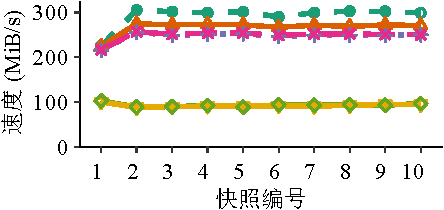
\includegraphics[width=0.47\textwidth]{pic/featurespy/plot/performance/LANTrace/trace_fsl.pdf}&
        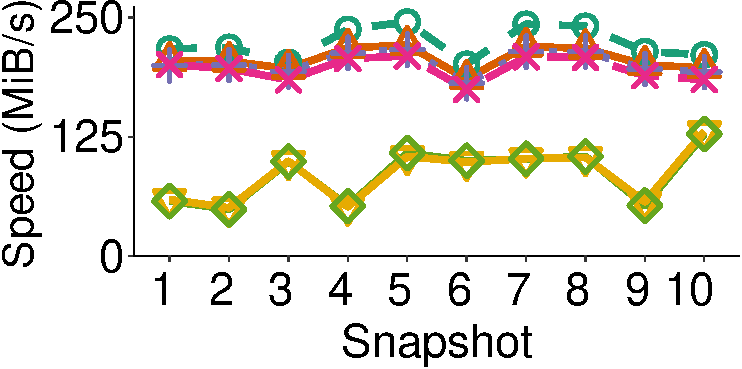
\includegraphics[width=0.47\textwidth]{pic/featurespy/plot/performance/LANTrace/trace_ms.pdf}\\
        \mbox{\small (a) FSL} &
        \mbox{\small (b) MS}\\
        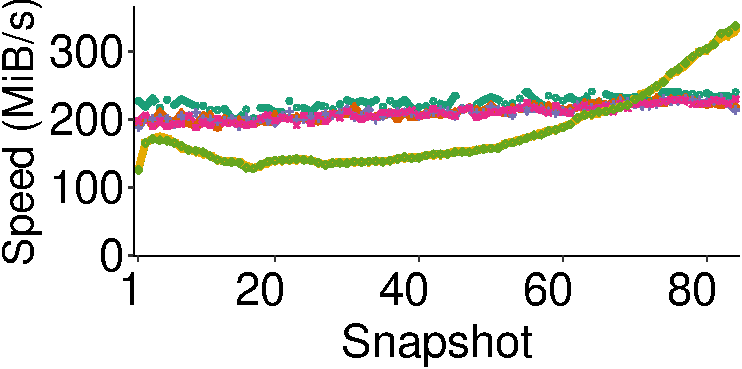
\includegraphics[width=0.47\textwidth]{pic/featurespy/plot/performance/LANTrace/trace_linux.pdf}&
        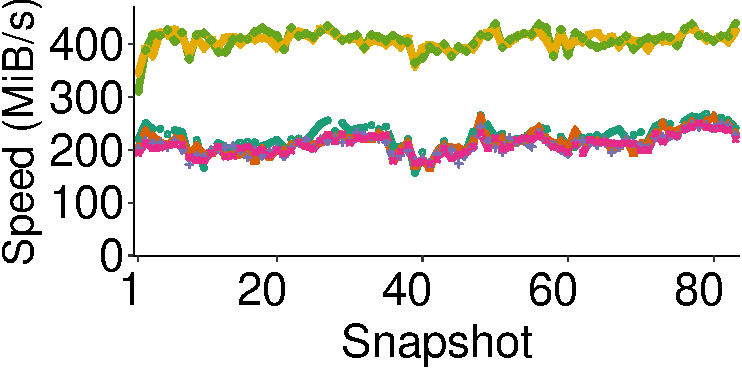
\includegraphics[width=0.47\textwidth]{pic/featurespy/plot/performance/LANTrace/trace_couch.pdf}\\
        \mbox{\small (c) Linux} &
        \mbox{\small (d) CouchDB}\\
    \end{tabular}
    \caption{(Exp\#9) Trace-driven performance.}
    \label{fig:featurespy-traceDrivenThroughput}
\end{figure}
图~\ref{fig:featurespy-traceDrivenThroughput} 展示了结果。在第一个 FSL 快照之后(例如,224.8\,MiB/s, 223.9\,MiB/s, 214.9\,MiB/s 和 216.9\,MiB/s 用于 \sysnameS、{\tt firstFeature}、{\tt minFeature} 和{\tt allFeature}),\sysnameS 和 \prototype 都实现了高性能(例如,至少 298.9\,MiB/s, 266.8\,MiB/s, 246.4\,MiB/s 和 248.8\,MiB/s \sysnameS、{\tt firstFeature}、{\tt minFeature} 和 {\tt allFeature}),因为它们不需要传输在 FSL 中占很大比例的交叉快照冗余。下载速度通常是稳定的(例如 \sysnameS 为 88.7-102.6\,MiB/s,\prototype 为 88.0-100.2\,MiB/s)。平均而言,与 \sysnameS 相比,{\tt firstFeature}、{\tt minFeature} 和 {\tt allFeature} 分别降低了上传性能 8.8\%、15.7\% 和 15.0\%,下载性能降低了 0.8 \%。

与 FSL 相比,MS 中的上传性能通常下降约 21\%,因为 MS 包含许多独特的块并导致较大的指纹索引(通过 LevelDB \cite{leveldb} 实现)。这加重了查询指纹索引是否存在密文数据块以进行重复数据删除的开销。此外,MS 中的下载速度会随着快照的变化而波动,因为一些快照具有更多的非重复块,并且可能存储在可以通过顺序读取快速访问的连续区域(即碎片较少的 \cite{lillibridge13})中。


\paragraph*{Exp\#10(网络流量分析)。}
本文分析了 \prototype 的网络流量,并将其与三种可以抵御推测内容攻击的重复数据删除方法进行比较:(i) {\em target-based deduplication} \cite{harnik2010side},强制客户端传输所有密文数据块到云服务端; (ii) {\em random-threshold deduplication} \cite{harnik2010side},如果每个块的上传次数小于预定义的阈值,则执行目标端重复数据删除,或源端重复数据删除 (\S\ref{sec:background-enc-deduplication}) 否则; (iii) {\em 两阶段重复数据删除} \cite{li15},它对来自同一客户端的密文数据块执行源端重复数据删除,然后对跨不同客户端的密文数据块执行目标端重复数据删除。在这里,本文按照之前的工作 \cite{harnik2010side} 分别在 20 和 2 处选择随机阈值重复数据删除中阈值的上限和下限。本文专注于 FSL 和 MS。对于 FSL,本文每天合并每个用户的快照,并按时间顺序存储。对于 MS,本文认为每个快照都来自一个单独的客户端,并按照快照 ID 的顺序存储快照。本文不考虑文件元数据导致的带宽开销。

\begin{figure}[!htb]
    \centering
    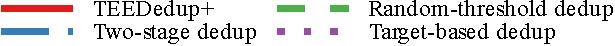
\includegraphics[width=0.8\textwidth]{pic/featurespy/plot/bandwidth/upload_traffic_legend.pdf}     \vspace{3pt} \\
    \begin{tabular}{@{\ }c@{\ }c}
        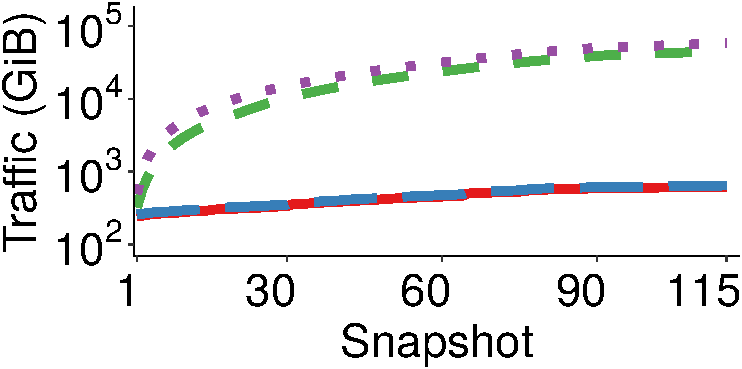
\includegraphics[width=0.47\textwidth]{pic/featurespy/plot/bandwidth/upload_traffic_fsl.pdf} &
        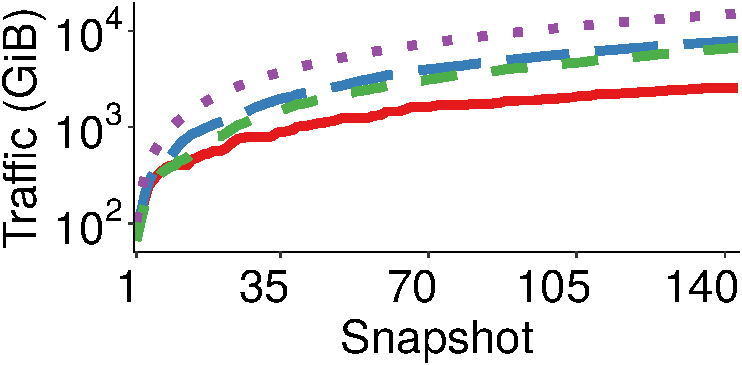
\includegraphics[width=0.47\textwidth]{pic/featurespy/plot/bandwidth/upload_traffic_ms.pdf} \\
        {\small (a) FSL} & {\small (b) MS} \\
        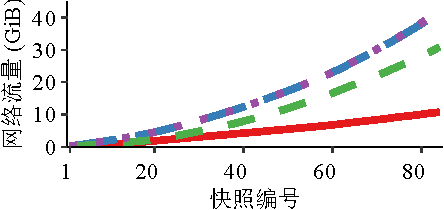
\includegraphics[width=0.47\textwidth]{pic/featurespy/plot/bandwidth/upload_traffic_linux.pdf} &
        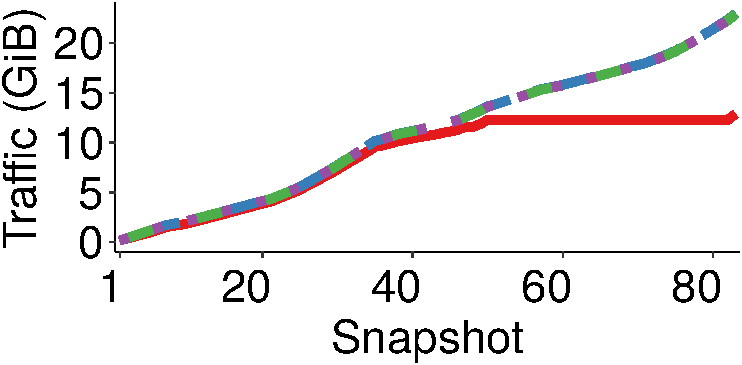
\includegraphics[width=0.47\textwidth]{pic/featurespy/plot/bandwidth/upload_traffic_couch.pdf} \\
        {\small (c) Linux} & {\small (d) CouchDB}
    \end{tabular}
    \caption{(Exp\#10) 存储每个快照后的累积网络流量。}
    \label{fig:featurespy-expNetworkTraffic}
\end{figure}

图~\ref{fig:featurespy-expNetworkTraffic} 展示了结果。由于 \prototype 执行纯源端重复数据删除,因此它优于其他方法。例如,在存储最后一个快照后,\prototype 将目标端重复数据删除的网络流量在 FSL 中减少了 98.9\%,在 MS 中减少了 83.1\%。两阶段重复数据删除在 ​​FSL 中表现良好(例如,只有 3.7\% 的带宽开销超过 \prototype),因为 FSL 包含大量用户内冗余。但是,在 MS 中,两级重复数据删除的网络流量最终是 \prototype 的 3.1$\times$。随机阈值重复数据删除会在 FSL(例如,\prototype 的 72.5$\times$)和 MS(例如,\prototype 的 2.6$\times$)中产生不同的网络流量。

由于 Linux 和 CouchDB 数据集的每个版本几乎没有冗余,并且需要大量源端重复数据删除查询,对于 Linux,它仅带来 $1.05\%$ 的流量节省,而对于 CouchDB,它甚至导致 $0.31 \%$ 额外的流量开销。随机阈值重复数据删除带来的流量节省是完全不同的。在 MS 中,它带来了 $55.75\%$ 的流量节省,而在 FSL 和 Linux 中,只有 $21.60\%$ 和 $26.68\%$。然而,它甚至在 CouchDB 中引入了 $0.0016\%$ 的额外流量开销。另外,本文发现在CouchDB的前35个版本中,几个方案的网络流量几乎是一样的,而对于后面的版本,\prototype 的累计网络流量几乎保持在一个水平。这是因为这 35 个版本是通用版本,几乎没有冗余。并且这些通用版本和社区/企业版本之间存在大量冗余,使得\prototype 不再需要上传大量数据。